\chapter{Data analysis for gravitational-waves from compact binary mergers}

In the previous chapter we discussed modeling GW signals from compact binaries, and in this chapter we will discuss  extremely sensitive observatories to detect fractional changes in length of $\mathcal{O}(10^{-21})$ and sophisticated data analysis techniques to find signals buried under large volumes of noisy data.  We will first give an overview of the ground based laser interferometers, along with an overview of the broad sources of noise in them. We will briefly talk about the existing observatories and those proposed for the future. Next, we will discuss the key components of data analysis techniques used for searching GW signals.    

%The indirect detection of gravitational waves (GWs) through the Hulse-Taylor binary pulsar represents a pivotal moment in astrophysics. Discovered in 1974 by Russell Hulse and Joseph Taylor, this binary system consists of a pulsar orbiting another neutron star. Over time, precise measurements of the pulsar's orbit exhibited a gradual decay in its orbital period. This decay matched predictions from Einstein's theory of General Relativity, which suggested that the system should be losing energy through the emission of gravitational waves. The energy loss rate, inferred from the changing orbital period, was found to be in excellent agreement with the theoretical predictions for gravitational wave emission. Although this was an indirect observation, it provided the first compelling evidence of the existence of gravitational waves and earned Hulse and Taylor the Nobel Prize in Physics in 1993. Their discovery not only confirmed a major prediction of General Relativity but also paved the way for future direct detections of gravitational waves. 


\section{Ground-based interferometers}
The earliest GW detectors were constructed by Joseph Weber (in 1960s) called as the \textit{Weber bar}, consisting of aluminum bar of 2 meters in length and a meter in diameter \cite{Weber:1960zz}. The Weber bars' principle idea for detection was using vibration at the resonance frequency of $\sim 1.6$ KHz. Resonant bars were not sensitive to detect any GWs and could only pick up signals with a strain around $\sim 10^{-16}$, which is significantly higher than the zero-order quadrupole strain of $h \sim 10^{-21}$ as calculated earlier. To put it in perspective, this level of sensitivity would only allow for the detection of a Binary Black Hole (BBH) merger occurring within a distance of about 1 kiloparsec (within our Milky Way), an event highly improbable given current estimates of such occurrences and conventional models of astrophysical binary populations \cite{Nitz:2021zwj,LIGOScientific:2021djp,Olsen:2022pin, Belczynski:2001uc,vandenHeuvel:2017pwp, Marchant:2016wow, Fragione:2018vty, Rodriguez:2017pec,Sedda:2020wzl}.

GWs cause matter to stretch in one direction while simultaneously squeezing the perpendicular direction. Leveraging this fundamental principle for detection, in the late 1960s a parallel effort kick started to make prototype interferometeric gravitational wave detectors. Over subsequent decades, extensive collaborative efforts across multiple fields – including instrumentation, engineering, and applied physics – were dedicated to enhancing the sensitivity of these massive interferometers. This combined effort made it possible to achieve the necessary precision to detect gravitational waves. In the next subsection, we briefly discuss the principle mechanism of interferometers required for detecting these waves. 


\subsection{LASER interferometers}
Today's ground-based GW observatories employ an evolved concept of a Michelson interferometer with the addition of a Fabry-Pe\'rot cavity. Currently there are five operational gravitational wave observatories: the Advanced Laser Interferometer Gravitational-Wave Observatory (LIGO) detectors in Hanford, (Washington), and Livingston, (Louisiana), in the United States \cite{LIGOScientific:2014pky}; Virgo, located near Pisa, Italy \cite{VIRGOdetector}; KAGRA, in Japan \cite{KAGRA:2018plz} and the GEO 600 in Sarstedt, Germany \cite{Dooley:2015fpa}. These detectors are part of a growing global network that collaborates to triangulate the source of gravitational waves and improve the sensitivity of detections. 


%The Advanced LIGO observatories in Hanford and Livingston are identical in their L-shaped design, with each arm being 4 kilometers long. The arms are kept in a near-perfect vacuum to minimize disturbances, and mirrors at the ends of each arm are suspended to isolate them from external vibrations. Virgo is a gravitational wave detector that features a 3-kilometer-long L-shaped interferometer. While slightly shorter than the LIGO arms, Virgo is crucial because of its longer duty cycle. KAGRA is unique among the ground based detectors as it is located underground in the Kamioka mine, which helps to shield it from seismic noise and provides a stable thermal environment. KAGRA uses a 3-kilometer-long L-shaped interferometer like Virgo and is designed to operate at cryogenic temperatures to reduce thermal noise. Despite its smaller size, GEO 600 compensates with advanced technologies, particularly in precision optics and LASER stabilization, making it a valuable test-bed for innovative techniques in gravitational wave detection. These advancements have often been instrumental in enhancing the sensitivity of the larger interferometers. 


\begin{figure}
    \centering
    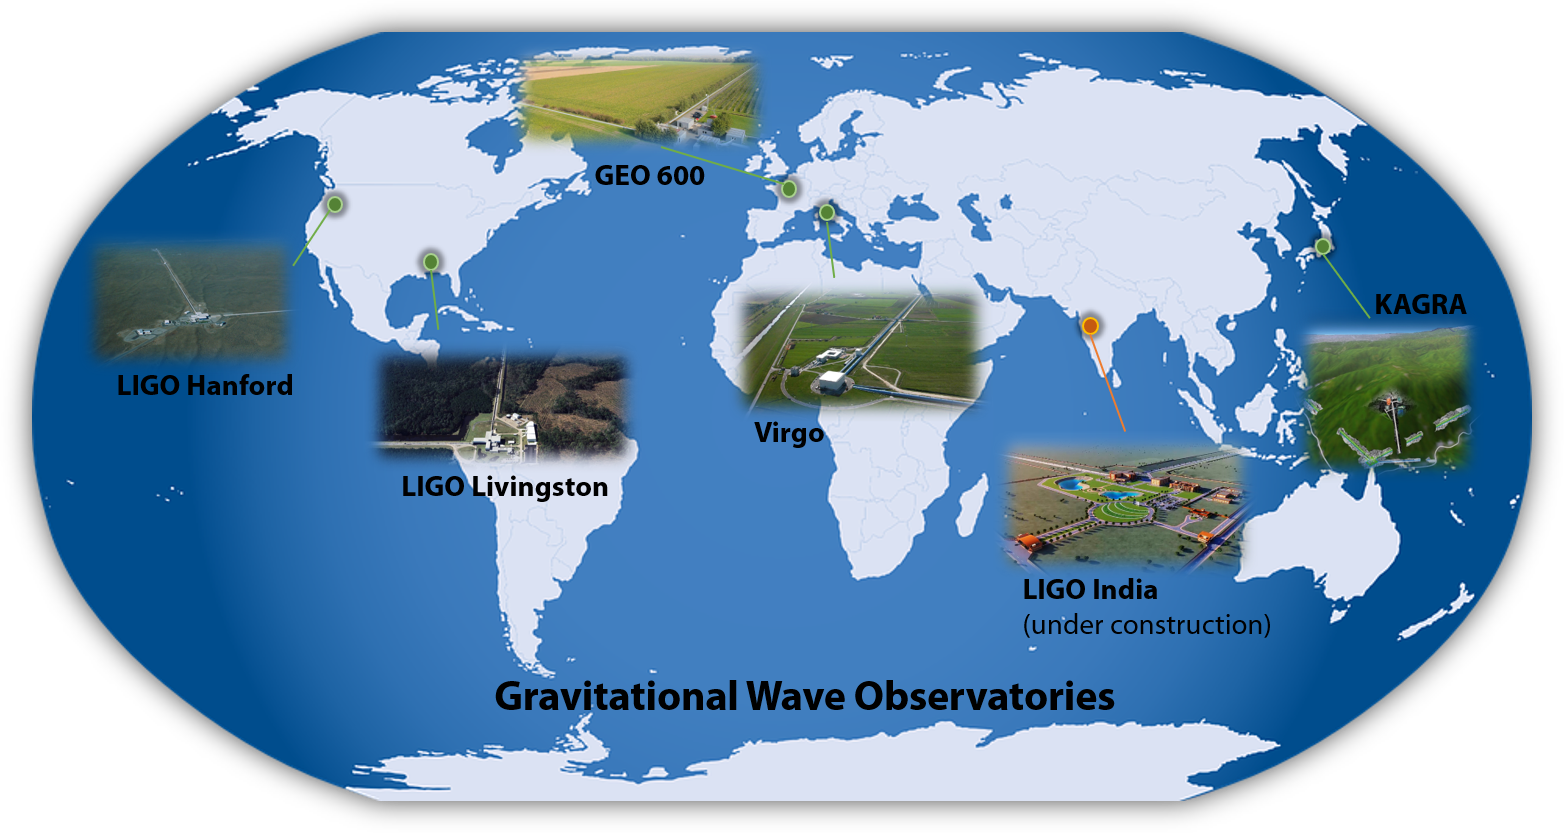
\includegraphics[width=\textwidth]{figures/basic_data_analysis/GW-observatories.png}
    \caption{Gravitational wave observatories around the World. LIGO Livingston and Hanford, Virgo and KAGRA contributing to scientific observing runs. The Advanced LIGO observatories in Hanford and Livingston are identical in their L-shaped design, with each arm being 4 kilometers long. Virgo is a gravitational wave detector that features a 3-kilometer-long L-shaped interferometer. KAGRA is unique 3-kilometer-long L-shaped interferometer, as it is located underground in the Kamioka mine. GEO600 is a nearly L-shaped interferometer with arm lengths of 600m, and serves as a key site to test technologies for the bigger observatories. Photo credits: LIGO, Joe Giaime, GEO600 and KAGRA.}
    \label{fig:GW-observatories}
\end{figure}


Michelson interferometer was successfully employed during the famed Michelson-Morley experiment in 1887 designed to verify the presence of an aether wind \cite{Michelson:1887zz}. In a simple Michelson interferometer (shown in Fig. \ref{fig:Michelson-interferometer}), a single beam of monochromatic light (usually a LASER) is directed towards a beam splitter. This mirror splits the beam into two separate but perpendicular paths: one continues straight while the other is reflected at a 90-degree angle. In normal conditions, without gravitational waves, these beams travel back and forth over the same distance and converge at the photodetector, resulting in destructive interference, effectively cancelling each other out. During the passing of an astrophysical GW signal will cause one arm of the interferometer to extend and the other to shrink (Fig. \ref{fig:Polarisation}). This alters the optical paths of the beams, leading to a time delay upon their return to the photodetector. Instead of cancelling out, they create a pattern of constructive interference. A photodetector is positioned at the output port to receive the beam and generate the readout. 
%This unique interference pattern serves as a detectable signature, characteristic of the astrophysical source of the gravitational wave. 

The interferometers measure ``strain", which is a dimensionless measure of the fractional change in length that one of the interferometer's arms experiences relative to the other. The minimum change in the interferometer's arm length is limited by the wavelength of the laser $\lambda_{\text{laser}} \sim \Delta L$. To the first order, the fractional change in the interferometer’s arm length is given by
\begin{align}
    \dfrac{\Delta L}{L} \simeq \dfrac{\lambda_{\text{laser}}}{L} \simeq 10^{-9}, 
    \label{Eq:rough-strain-sensitivity}
\end{align}
using arm lengths $\mathcal{O}$(1 km) and lasers with wavelength $10^{-6}$m. In comparison,  typical GW strain is $\sim 10^{-21}$ (using Eqs. (\ref{Eq:ring-eqn}) and (\ref{Eq:toymodel-plus})), several orders of magnitude smaller than what could be detected by a simple Michelson interferometer.  
%We can write the phase difference accumulated with a LASER of wavelength $\lambda_l \sim 1 \mu m$, as \cite{Maggiore:2008aaa} 
%begin{align}
%    \Delta \Phi = \dfrac{4\pi}{\lambda_L}h_+L \sim 10^{-12}.  
%\end{align}

To improve the inteferometer's ability to reach required sensitivity, additional components are employed that increase the effective path length and power of the laser. The light from beam splitter is trapped inside a \textit{Fabry-P\'erot} \cite{Maggiore:2008aaa} cavity (two parallel, highly reflective mirrors), allowing it to bounce back and forth -- increasing the effective distance travelled by each laser from $4$km to $\sim 1000$km. Increasing the power of the laser also improves the performance of the interferometer -- more number of photons leads to sharper fringes at the photodetector. To achieve this, a \textit{power recycling mirror} is used to reflect the laser light that has already passed through the instrument, back into the interferometer, effectively `recycling' it \cite{Meers:1988wp}. This continuous cycling of laser power, coupled with the constant influx of light from the laser source, significantly enhances laser light's power inside the interferometer without the necessity of initially producing an extremely powerful laser beam. A similar technique is used to recycle the power of the light before it reaches to the photodetector, called \textit{signal recycling} \cite{Buonanno:2001cj}. 

These enhancements allow the interferometers to reach the sensitivity of $h \sim 10^{-21}$. At such small length deviations, numerous factors impact the movement of the test masses and the detectable output signal, acting as noise that constrains the detectors' sensitivity. These noise sources are largely well-characterized and can be effectively modeled, as discussed next. 

\begin{figure}
    \centering
    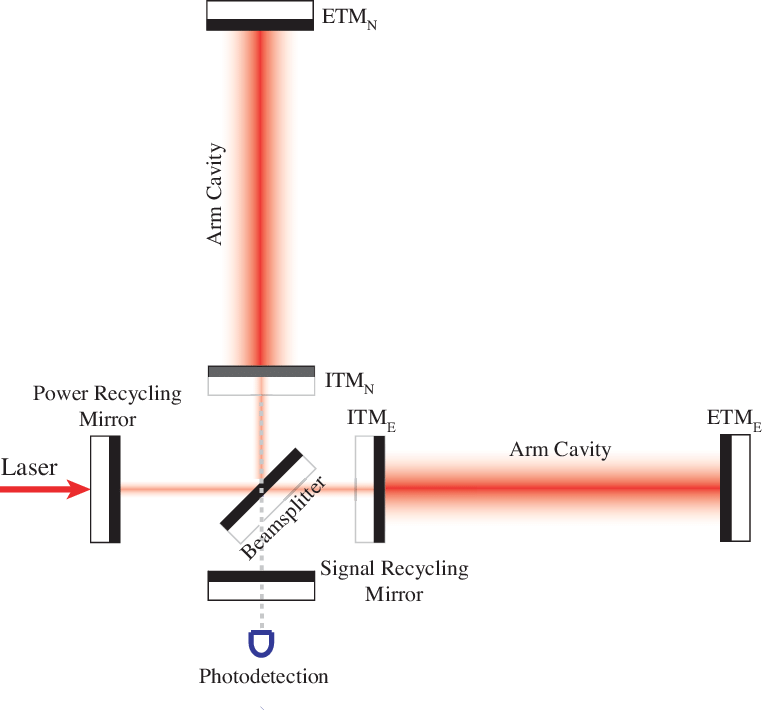
\includegraphics[width=0.5\textwidth]{figures/basic_data_analysis/Michelson-interferometer.png}
    \caption{A simplified design of a LASER interferometer: The left panel presents a basic diagram of a LASER interferometer with its arms aligned along the $x$ and $y$ axes. A beam splitter divides the incoming laser light, directing it into two arms, each housing a Fabry-Pérot cavity. These beams are then merged back together and captured at the output. Image credits: \cite{Kondrashov:2008zr}}
    \label{fig:Michelson-interferometer}
\end{figure}

\subsection{Noise sources}
Achieving the extraordinary sensitivity means that these detectors have to deal with a plethora of noise sources that can mask or mimic gravitational-wave signals.  To keep track of the detector's internal condition and its surrounding physical environment, a variety of additional sensors are employed, gathering data through auxiliary channels. Below is an expanded look at the main types of noise that affect ground based gravitational wave observatories:

Quantum noise in gravitational wave detectors arises from the Heisenberg uncertainty principle, which limits the precision with which pairs of physical properties, like position and momentum, can be known. A technique called \textit{squeezing} is used to swap the uncertainties in the measurement of amplitude or phase of the noise, which is related by the Heisenberg uncertainity principle \cite{Oelker2016}. 
\begin{itemize}
    \item Shot Noise: This is a form of quantum noise that arises because light consists of discrete particles (photons). When measuring the interference pattern in an interferometer, the discrete arrival of photons causes statistical fluctuations in the detected light intensity. At high laser power, shot noise predominates and limits the high-frequency sensitivity of the detectors \cite{Tse2019}.
    \item Radiation Pressure Noise: At lower frequencies, the variability is dominated by radiation pressure noise. This is the fluctuation in force exerted by photons as they bounce off the mirrors. It introduces a quantum limit to the low-frequency sensitivity due to the momentum transfer of the light \cite{Kondrashov:2008zr}.
\end{itemize}

The inherent Brownian motion of the atoms in any macroscopic object at a given temperature generates thermal noise. This effect impacts both the mirrors and the suspension system \cite{Levin:1997kv}:
\begin{itemize}
    \item Suspension Thermal Noise: The motion of the suspension fibers can introduce noise due to thermal vibrations. Advanced detectors use materials such as fused silica with very low mechanical losses to suspend the mirrors, minimizing this source of noise \cite{Aston:2012ona}.
    \item Mirror Thermal Noise: The mirrors themselves are also sources of thermal noise. Brownian motion within the reflective coating and the substrate material of the mirrors can lead to fluctuations in the reflected light phase \cite{Braginsky:2003yhs}. Lowering temperatures (as with KAGRA) can reduce such noise \cite{Steinlechner:2018crl}. Additionally, the Brownian noise of the mirror coatings also has a non-negligible impact, which can be reduced by using improved AlGaAs coatings (as planned for future observatories) \cite{Cole:2023sak}.  
\end{itemize}

Seismic noise is the result of ground vibrations transmitted through the Earth, originating from natural and anthropogenic sources: 
\begin{itemize}
    \item Ground Vibrations: These are the primary source of noise below a few tens of hertz. They can be caused by earthquakes, ocean waves, or even nearby human activity such as traffic or industrial work. Advanced isolation systems are used to minimize this noise, including active seismic isolation, which uses sensors to detect ground motion and actuators to counteract it, and passive isolation, such as layers of springs and masses that absorb vibrations \cite{Aston:2012ona,Daw:2004qd}.
\end{itemize}

Gravity gradient noise, also known as Newtonian noise, is due to fluctuations in the local gravitational field \cite{Harms:2015zma,Saulson:1984yg}:
\begin{itemize}
    \item  Environmental Factors: These can be caused by atmospheric pressure changes, density changes in the Earth, or even human activity, all of which can create varying gravitational forces on the detector components. This type of noise is particularly challenging to mitigate because it cannot be shielded against in the same way as electromagnetic noise. Efforts to subtract it involve modeling the environmental effects and removing their signature from the data \cite{Harms:2020uyc}.
\end{itemize}

Instrumental noise arising from the detector components:
\begin{itemize}
    \item  Electronic Noise: In the photodetectors and other electronic systems, inherent noise can be introduced. This is typically white noise that can be well-characterized and filtered \cite{Kondrashov:2008zr}.
    \item Calibration Errors: Uncertainty in the detector's response to gravitational waves can also introduce noise into the measurement. Regular calibration is necessary to minimize this noise \cite{Sun:2020wke}.
\end{itemize}

Despite efforts to correlate noise with auxiliary channels, numerous types of short noise artefacts \textit{glitches} remain persistent in the data which reduce our confidence for detection by mimicking GW signals. Certain types of transient noises, namely Blips, Tomte, and Koi-Fish, have been observed to happen at a frequency of about once per hour \cite{Cabero:2019orq}. To date, these glitches have not been definitively linked to any environmental or instrumental causes \cite{Cabero:2019orq}. Eradication of glitches require additional vetoeing technqiues while searching for GW signals, which will be discussed later in this chapter.  

\begin{figure*}
    \centering
    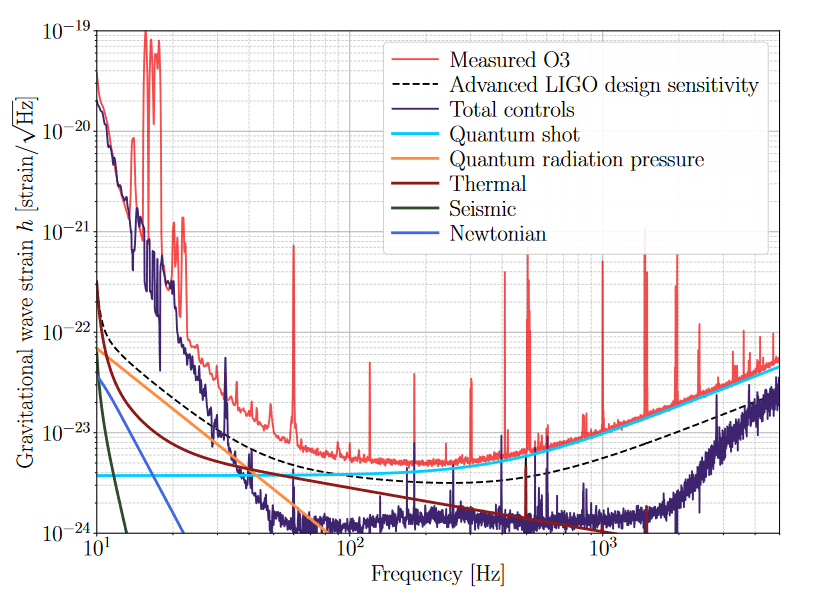
\includegraphics[width=\textwidth]{figures/basic_data_analysis/O3_noise_budget.PNG}
    \caption{O3 noise budget. Only few noise sources are shown for a simplified picture. Image credits: \cite{aLIGO:2020wna}}
    \label{fig:O3_noise_budget}
\end{figure*}



\subsubsection{Upcoming and future observatories}

There are two upgrades planned for the current Advanced LIGO observatories for the post-O5 timeline -- LIGO A+ and LIGO $\text{A}^{\#}$. LIGO A+ is expected to be $2\times$ more sensitive than Advanced LIGO and would involve improvements such as better seismic noise isolation and test mass suspensions \cite{KAGRA:2013rdx}. Further factor of two improvement is expected with LIGO $\text{A}^{\#}$ with reduction in quantum noise and coating thermal noise \cite{Asharp}.

%.  LIGO $\text{A}^{\#}$, is the upgrade further aimed towards boosting sensitivity the following O5 observation run, slated for 2029. This upgrade is designed to fill the observational gap and maintain continuity in gravitational wave research until the third-generation facilities, such as the Cosmic Explorer and Einstein Telescope, become operational.

Third-generation (3G) gravitational wave detectors, such as the Cosmic Explorer and the Einstein Telescope are planned to become operational by mid 2030s \cite{Gupta:2023lga,Punturo:2010zz}. The Cosmic Explorer, with its proposed arm lengths of up to 40 kilometers, aims to increase up to an order of magnitude in sensitivity and observational range over current detectors \cite{Evans:2021gyd}. The Einstein Telescope, planned to be an underground facility in Europe with a triangular configuration of 10-kilometer arms, seeks to reduce seismic noise and enhance detection capabilities \cite{Hild:2010id}. The location of both the 3G observatories is not yet finalized, but is strongly preferred to be in the USA for CE and in Europe for ET. 

Ground-based interferometers are limited by seismic noise, especially at frequencies below one Hertz. To circumvent this, efforts have shifted to space-based interferometers, such as the Laser Interferometer Space Antenna (LISA) \cite{LISA:2017pwj}. A collaborative project between the European Space Agency and NASA, LISA is set for a 2030s launch \cite{LISA-intro, LISA:2017pwj, eLISA:2013xep} after the success of the test mission LISA Pathfinder \cite{Armano:2016bkm,McNamara:2008zz}. LISA will consist of three spacecraft forming a vast triangle, each side stretching 2.5 million kilometers, in space. LISA's science case is rooted in its potential to open new windows for new source like Extreme Mass Ratio Inspirals (EMRIs), Intermediate Mass BBHs (IMBBH) mergers, galactic binary inspirals and cosmological stochastic background \cite{eLISA:2013xep}. The noise curves for various GW observatories mentioned above are shown in the Fig. (\ref{fig:Gw-plotter}).

\begin{figure}
    \centering
    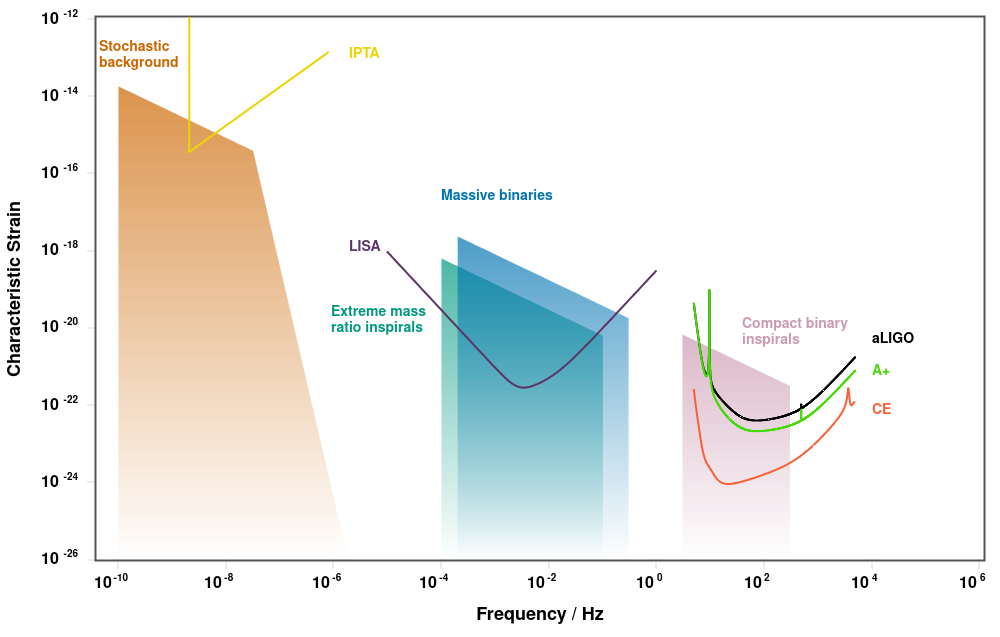
\includegraphics[width=\textwidth]{figures/basic_data_analysis/Gw-plotter.png}
    \caption{Sensitivity curves and expected strains: Bold lines show predicted senstivity curves for various GW detectors, including ground based Advanced LIGO observatory, space based LISA and International Pulsar Timing Arrays. Senstivity curves for some proposed observatories for the future -- A+, Cosmic Explore, LISA are also shown. The shaded regions show characteristic strain for various sources as labelled. Source: \href{http://gwplotter.com/}{GW-plotter}.}
    \label{fig:Gw-plotter}
\end{figure}

\subsubsection{Signal observed at a ground based detector}
In Eqs. (\ref{Eq:toymodel-plus}) and (\ref{Eq:toymodel-cross}), we performed the transformation of gravitational radiation from the source to the radiation frame. An additional projection of the signal is necessary due to the detector's varying sensitivity across different sky points. This involves transforming the signal to the detector frame using three Euler angles, determined by the sky location of the source $(\alpha,\delta)$ known as the declination and right ascension and the polarization angle $\psi$ which signifies the rotation of the wavefront along the line of sight. The signal observed at the detector is then written in terms of the linear combination of the two polarizations
\begin{align}
    h(t) = F_+h_+ + F_{\times}h_{\times},
    \label{Eq:}
\end{align}
where the co-efficients are the \textit{antenna pattern functions} of the detector as shown in the Fig. \ref{fig:antenna-pattern}, and are given by \cite{Schutz:2011tw}
\begin{align}
    F_{+}(\alpha,\delta,\psi) = -\dfrac{1}{2}(1+\cos^2\alpha)\cos 2\delta\cos 2\psi -\cos\alpha\sin 2\delta\sin 2\psi, \\
    F_{\times}(\alpha,\delta,\psi) = \dfrac{1}{2}(1+\cos^2\alpha)\cos 2\delta\sin 2\psi -\cos\alpha\sin 2\delta\cos 2\psi.
    \label{Eq:det-frame-signal}
\end{align}


\begin{figure}
    \centering
    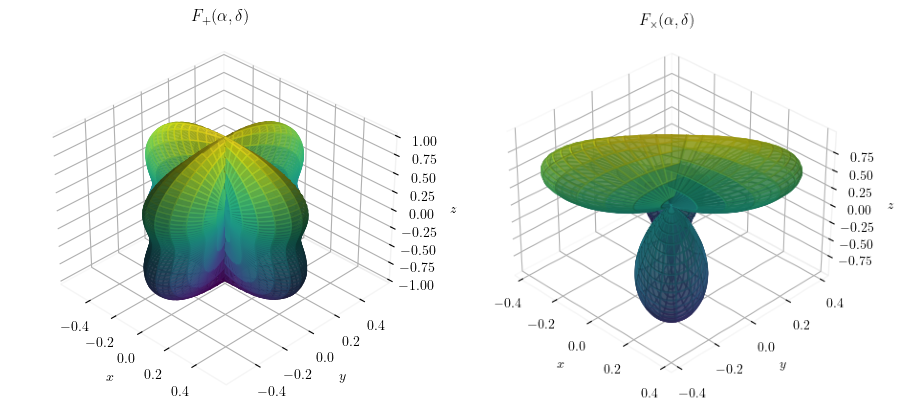
\includegraphics[width=\textwidth]{figures/basic_data_analysis/antenna-pattern.png}
    \caption{Angular distibution of the antenna pattern functions of an observatory in the $x-y$ plane.}
    \label{fig:antenna-pattern}
\end{figure}


\subsection{Basics of Fourier domain analysis}

Fourier domain analysis is a mathematical technique widely used in the field of data analysis to extract signal information from noisy data. Gravitational-wave signals are often buried in noise, making it difficult to detect them in the time domain. However, by transforming the data into the frequency domain using Fourier analysis, it becomes easier to identify and analyze these signals.


Suppose we have a function of time $x(t)$. Let us denote the Fourier transform of $x(t)$ by $\tilde{x}(f)$, which is given by
    \begin{align}
        \tilde{x}(f) = \int_{-\infty}^{\infty} e^{-2\pi i ft} x(t) dt,
    \end{align}
    similarly, the inverse Fourier transform is given by
    \begin{align}
        x(t) = \int_{-\infty}^{\infty} e^{2\pi i f t} \tilde{x}(f) df.
    \end{align}

\subsubsection{Discrete Fourier Transform}
Continuous signals $x(t)$ are analyzed by sampling at discrete intervals of $\Delta t$ to create a finite set of data points $x[t_i]$. If this signal is band-limited to a maximum frequency $f_{max}$, then the sampling interval $\Delta t$ is determined by adhering to the \textit{Nyquist-Shannon} sampling theorem \cite{Nyquist-shannon} -- the sampling frequency $f_s \equiv 1/\Delta t > 2f_{max}$. We can then write the Discrete Fourier Transform (DFT) of $x[t]$ assuming $N$ samples, as
\begin{align}
    \tilde{x}[f_k] = \Delta t \sum_{j=0}^{N-1} x[t_j] e^{-2\pi i j k/N},
\end{align}
and similarly the Inverse DFT as
\begin{align}
    x[t_k] = \Delta f \sum_{j=0}^{N-1} \tilde{x}[f_j] e^{2\pi i j k/N},
\end{align}
where $\Delta f \Delta t = 1/N$.

The DFT assumes that the input sequence is one period of a periodically repeating signal. This implies that the DFT treats the data as if it were part of a periodic sequence. The direct computation of DFT requires $O(N^2)$ operations, which can be expensive for large number of samples. 

The Fast Fourier Transform (FFT) most famously in the form of the Cooley-Tukey algorithm to reduce the computational complexity of the DFT \cite{Cooley-Tukey}.  The FFT algorithm exploits the periodicity and symmetry of the complex exponential function to reduce redundancy in computations, applying the algorithm recursively to increasingly smaller DFTs, and then efficiently combining these results which reduces the complexity to $O(N\log N)$.


\subsection{Modeling and measuring the noise}
The noise time series in a detector like LIGO is a complex superposition of various stochastic processes. We represent this time series $n(t)$ as a vector $\textbf{n}$ (or random process), where each of the discrete samples $n_i = n(t_i)$ is described as random variable with values according a probability distribution $p_i = p(n_i)$. The complete noise vector is then associated to to a joint probability distribution $p(\textbf{n})$. 

Features of any probability distribution can be captured by measuring moments. The first two moments of a stochastic process are often of particular interest -- mean $\mu = \langle \textbf{n}\rangle$ and covariance $C_{ij} = \langle(n_i-\mu)(\mu-n_j)\rangle$, where $\langle\rangle$ is defined as the expectation value of a random variable over time. The ensemble average is equivalent to a long time average. We can estimate these two quantities from the data with $N$ data samples uniformly sampled with sampling interval $\Delta T$
\begin{align}
    \mu = \dfrac{1}{N}\sum_{i=1}^{N}n_{i}.
    \label{eq:mean-noise-series}
\end{align}
And, the covariance matrix can be estimated using
\begin{align}
    C_{ij} = \langle (n_{i} - \mu)(\mu - n_j) \rangle.
    \label{eq:covariance-noise-series}
\end{align}
The covariance matrix allows us to estimate the \textit{power spectrum} which is essential in characterizing the noise. The power spectrum can be shown to be the expectation value of $n^2$ over a large duration of time interval $T$,
\begin{align} 
   \langle n^2 \rangle &= \lim_{n\to\infty} \dfrac{1}{T} \int_{-\infty}^{\infty} |n_T(f)|^2 df,\\
   & = \int_0^{\infty} S_n(f) df,
\end{align}
where $n_T(t) = n(t)w_T(t)$ is a windowed signal within $-T/2 < t < T/2$ and $S_n(f)$ is the \textit{power spectral density} of the process $n(t)$ (we refer the reader to \cite{Allen:2005fk} for a detailed derivation). Now, we model the noise by assuming zero mean and by using three properties that will help characterize the noise better, these properties are: 

\subsubsection{Stationary}
A stochastic process is known as wide-sense \textit{stationary} process where the statistical properties are invariant with time. Specifically, for a process to be considered wide-sense stationary, it must satisfy two main conditions: 1. the mean of the process is constant over time and 2. the covariance function $C_{ij}$ depends only on the time difference (lag) and not on the specific time. Using the stationarity conditions, the covariance matrix can be written as
\begin{align}
    C(n(t), n(t+\tau)) = \langle n(t)n(t+\tau) \rangle = R_n(\tau),
\end{align}
for all $t$ and $\tau$, where the \textit{autocorrelation function} $R_n(\tau)$ is the correlation between a signal with a delayed copy of itself.

Assuming the noise process to be wide-sense stationary, the power spectral density can be related by the \textit{autocorrelation} function $R_n(\tau)$ using the Wiener-Khinchin theorem as
\begin{align}
    S_n(f) := \int_{-\infty}^{\infty} R_n(\tau)e^{- i2\pi f\tau} d\tau.
    \label{Eq:Weiner-Khinchin}
\end{align}

Another useful property of power spectral density in the Fourier domain is that the expectation value of two frequency components $\tilde{x}(f)$ and  $\tilde{x}(f')$ is proportional to the Dirac delta function $\delta(f-f')$
\begin{align}
    \langle \tilde{n}^*(f') \tilde{n}(f) \rangle = \dfrac{1}{2}S_n(f)\delta(f-f').
    \label{Eq:PSD-prop-fourier}
\end{align}

%where $\tau$ is the lag, or the time difference between the signal and its delayed version. For noise process with zero mean, it can be shown from Eq. () that the covariance matrix is the same as the autocorrelation function
%\begin{align}
%    C(\tau) = R_n(\tau) \hspace{1cm} \text{for} \hspace{1cm} (\langle \textbf{n} \rangle = 0).
%\end{align}

\subsubsection{Colored}
We first consider a simple case of white noise, which is characterized by a constant power spectral density across all frequencies within a given bandwidth. This means that every frequency component has the same power
\begin{align}
    S_n(f) = S_0.
\end{align}
In case of white noise, the covariance matrix is a constant $C_{ij} = S_0/\Delta t$, where $\Delta t$ is the sampling interval.

Colored noise has a PSD that changes depending on the frequency. This variation can take different forms, such as $S_n(f) \propto 1/f$ known as pink noise. Using $S_n(f)$ as the PSD for a stationary colored noise, the covariance matrix is diagonalized and can be written as
\begin{align}
    C_{ij} = S_n(f_i)\delta_{ij}
    \label{Eq:Colored-noise-PSD}
\end{align}
 
\subsubsection{Gaussian}

This property allows us to write the joint probability distribution of noise time-series $p(\textbf{n})$ with $N$ samples, following a multi-variate normal distribution using the mean and covariance matrix described above 
\begin{align}
    p(\textbf{n}) = \dfrac{1}{(2\pi)^{N/2}\sqrt{\text{det}(\textbf{C})}}\text{exp}\Bigg[-\dfrac{1}{2} \sum_{ij}n_{i}C_{ij}^{-1}n_j  \Bigg],
    \label{Eq:joint-pdf-noise}
\end{align}
where $C_{ij}^{-1}$ represents the inverse and $\det(\textbf{C})$ the determinant of the covariance matrix. We define the matrix $G_{ij}$ as the inverse of the covariance matrix, which is given by $G_{ij} = 1/S_n(f)$. Using Eq. (\ref{Eq:joint-pdf-noise}), we can simplify the exponent part of the joint probability distribution 
\begin{align}
    p(\textbf{n}) & \propto \exp \Bigg[ - \dfrac{1}{2} \sum_{ij} \dfrac{n_i \delta_{ij} n_j}{S(f)} \Delta t \Bigg]\\
    &  \propto  \exp \Bigg[ - \dfrac{1}{2} \int_{0}^{T} \dfrac{n(t)^2}{S(f)} dt \Bigg] \\
    &  \propto  \exp \Bigg[ - \dfrac{1}{2} 4\int_{0}^{\infty} \dfrac{|\tilde{n}(f)|^2}{S(f)} df \Bigg],
\end{align}
where we have used that $n(t)$ is real-valued implying $\tilde{n}(-f) = \tilde{n}^*(f)$.

Defining a noise-weighted inner product between two time series $x(t)$ and $y(t)$ as,
\begin{align}
    (x|y) := 4 \Re \int_{0}^{\infty} \dfrac{\tilde{x}(f)\tilde{y}^*(f)}{S_n(f)} df,
    \label{Eq:inner-product}
\end{align}
we can write the probability density for a stationary Gaussian colored noise process $n(t)$ concisely as,
\begin{align}
    p(\textbf{n}) \propto e^{-(\textbf{n}|\textbf{n})/2}.
    \label{Eq:noise-probability}
\end{align}

\section{Optimal method to extract signal out of noise: Matched-filtering}

Matched-filtering technique is at the heart of modeled approaches for detecting compact binary coalescence (CBC) signals. This technique is performed in the Fourier domain, which estimates the probability of a stretch of data containing an anticipated signal $\tilde{h}(f)$ within Gaussian noise. The statistic used in matched-filtering is essentially a correlation involving the Fourier-transformed data $\tilde{s}(f)$ and a template $\tilde{h}(f)$ weighted by the noise power spectral density (PSD) $S_n(f)$. The complex matched-filter statistics is defined as 
\begin{align}
    \label{Eq:complex_matched_filter}
    \braket{s|h} = 4\int_{0}^{\infty} \dfrac{\tilde{s}(f)\tilde{h}^*(f)}{S_n(f)},
\end{align}
and the real component of this complex matched-filter is same as the inner product defined in Eq. (\ref{Eq:inner-product})
\begin{align}
    (s|h) = \Re [\innerproduct{s}{h}].
\end{align}
We define the output of the matched-filter as the signal-to-noise ratio (SNR)
\begin{align}
    \label{Eq:SNR_def}
    \rho^2 \equiv \dfrac{(\Real[\braket{s|h}])^2}{\braket{h|h}} = \dfrac{(s|h)^2}{(h|h)}.
\end{align}

We can show the matched-filter is an optimal detection statistic which maximizes the SNR, by invoking the Neyman-Pearson criterion \cite{Wainstein1963}. This criterion maximizes the probability of correctly rejecting a false null hypothesis (true positive) at a given probability of incorrectly rejecting a true null hypothesis (false positive). 

We assume the strain data $s(t)$ contains noise process $n(t)$ with or without a possible GW signal with known form $h(t)$, to construct two hypotheses:
\begin{align}
    \text{Null Hypothesis} \hspace{1em} \mathcal{H}_0 :  & s(t) = n(t), \\
    \text{Alternate Hypothesis} \hspace{1em} \mathcal{H}_1 : & s(t) = h(t) + n(t).
\end{align}
Assuming Gaussian noise, we can then compute the probability density for each hypothesis as (from Eq. (\ref{Eq:noise-probability}))
\begin{align}
    p(s|\mathcal{H}_0) & \propto e^{-(s|s)/2},\\
    p(s|\mathcal{H}_1) & \propto e^{-(s-h|s-h)/2}.
\end{align}
Then using Bayes's theorem we can write the likelihood ratio as
\begin{align}
    \Lambda(\mathcal{H}_1|s) = \dfrac{p(s|\mathcal{H}_1)}{p(s|\mathcal{H}_0)},
\end{align}
and substituting the probabilities for the two hypothesis to get the log-likelihood ratio as
\begin{align}
    \log\Lambda(\mathcal{H}_1|s) = (s|h) - \dfrac{(h|h)}{2}.
\end{align}
Now, suppose if the signal as an unknown amplitude $h(t) = Ah_0(t)$, then we can maximize the log-likelihood ratio over this parameter to get
\begin{align}
    \max_{A} [\log\Lambda(\mathcal{H}_1|s)] = \dfrac{(s|h_0)^2}{(h_0|h_0)} = \dfrac{\rho^2}{2}
\end{align}
which is related to the matched filter SNR from Eq. (\ref{Eq:SNR_def}).

%which is a monotonically increasing function of the data $s(t)$ only via the term $(s|h)$.  

%It can be shown that matched-filter provides the optimal statistical measure, by maximizing the signal-to-noise ratio (SNR) \cite{Maggiore:2008aaa,Creighton-book}
%The signal-to-noise (SNR) ratio $\rho$ which is the matched-filter output maximised over an overall amplitude,   

%This technique scans through data from interferometers to identify patterns that match the anticipated GW signal waveform $\tilde{h}(f)$. This technique is performed in the frequency domain to detect the anticipated GW signal, denoted as $\tilde{h}(f)$, commonly referred as the \textit{template}. 

%Knowing the statistical characteristics of the noise and the precise nature of the signal enables the creation of an optimal detection statistic, which quantifies the likelihood that the data includes the expected signal.




%and the likelihood depends on the data only via the inner products $(s|h)$ and $(h|h)$. 
%Thus the noise-weighted inner product, called as \textit{matched-filtering} is the optimal detection statistic.

%The mathematical expression for the complex matched-filter statistic is:


\subsection{Unknown signal parameters}\label{sec:MF-maximization}
The previous section dealt with calculating the optimal statistic for known GW signals or those differing only in amplitude. In practice, the signal parameters are unknown a priori,  necessitating the maximization of SNR across the entire parameter space of astrophysical signals. We simplify the signal parameter space by assuming quasi-circular systems with only the dominant ($2,2$) mode of the GW emission which are described by 15 distinct parameters. We categorize the parameters into two groups: (1) intrinsic parameters $\vec{\zeta}$ -- the component masses $(m_1, m_2)$ and three-dimensional spin vectors $(\vec{\chi_1}, \vec{\chi_2})$, and (2) extrinsic parameters $\gamma$, that are defined from the perspective of the observer, these are: the standard spherical coordinates -- distance and inclination of the source, the reference orbital phase at coalescence $(d_L, \iota, \Phi_c)$, position in the sky $(\alpha, \delta)$, polarization $\psi$, and the coalescence time $t_c$.

Searching over a broad range of sources over the complete 15-dimensional parameter space is computationally challenging. A simplified procedure is to invoke analytical approximations that help reduce the problem to fewer variables. To demonstrate this procedure, we begin with the signal seen by the detector in Fourier domain is given by, 
\begin{align}
    \tilde{h}(f) &= F_{+}(\alpha,\delta,\psi)\tilde{h}_{+}(\vec{\zeta}, d_L,\iota;f) + F_{\times}(\alpha,\delta,\psi)\tilde{h}_{\times}(\vec{\zeta}, d_L,\iota;f).
\end{align}
We can simplify the signal by combining $F_+$ and $F_{\times}$ and using normalized templates 
\begin{align}
    \hat{h} = \dfrac{\tilde{h}}{\innerproduct{\tilde{h}}{\tilde{h}}^{1/2}}.
\end{align}
The above equation allows us to freely scale the amplitude of the templates. Writing the templates and antenna pattern functions by omitting the parameters for the sake of brevity, we get
\begin{align}
    \tilde{h} &= A(u\hat{h}_+ + \hat{h}_{\times}), 
    \label{Eq:detector-signal-fourier-domain}
\end{align}
where
\begin{align}
    u = \dfrac{F_{+}}{F_{\times}}\sqrt{\dfrac{\innerproduct{\hat{h}_{+}}{\hat{h}_{+}}}{\innerproduct{\hat{h}_{\times}}{\hat{h}_{\times}}}},
\end{align}
and
\begin{align}
    A = F_{\times}\sqrt{\innerproduct{\hat{h}_{\times}}{\hat{h}_{\times}}}.
\end{align}
Inserting the Eq. (\ref{Eq:detector-signal-fourier-domain}) into (\ref{Eq:SNR_def}), the amplitude term gets cancelled. Maximising SNR over $u$ results into \cite{Harry:2017weg}
\begin{align}
    \max_{u}(\rho^2) = \dfrac{(s|\hat{h}_{+})^2 +
                            (s|\hat{h}_{\times})^2 
                            - 2(s|\hat{h}_{+})(s|\hat{h}_{\times})(\hat{h}_+|\hat{h}_{\times})}{\Big(1-(\hat{h}_+|\hat{h}_{\times})^2\Big)}.
    \label{Eq:Generic-SNR-maximization}
\end{align}

Eq. (\ref{Eq:Generic-SNR-maximization}) indicates the SNR maximization problem reduces to only the intrinsic parameters ($\vec{\zeta}, \iota, \Phi_c$ and $t_c$). Assuming the component spins to be aligned with the orbital angular momentum and by searching only using the dominant gravitational-wave mode, we get  
\begin{align}
    \hat{h}_{+} \propto i\hat{h}_{\times},
    \label{Eq:polarization-symmetery}
\end{align}
which implies $\innerproduct{\hat{h}_+}{\hat{h}_{\times}} \simeq 0$. The above approximation further simplifies the Eq. (\ref{Eq:Generic-SNR-maximization}) to just one polarization. Maximization of $\Phi_c$ can be done over a quadrature by taking the absolute value of the complex SNR
\begin{align}
    \max_{d_L,\alpha, \delta, \psi, \iota, \Phi_c}(\rho^2) \simeq \norm{\innerproduct{s}{\hat{h}_+}}^2.
    \label{Eq:Simple-SNR-maximization}
\end{align}
The above statistics maximizes the SNR over the parameters ($d_L, \alpha, \delta, \psi, \iota$ and $\Phi_c$) in terms of a fiducial amplitude and phase. We remind the reader that Eqs. (\ref{Eq:polarization-symmetery}) and (\ref{Eq:Simple-SNR-maximization}) may not be valid for systems with arbitrary spins or eccentric orbits or with significant subdominant GW mode emissions.


The remaining four parameters are maximized using a discrete grid of points sufficiently covering the four dimensional parameter space $(m_1, m_2, \chi_{1z}, \chi_{2z})$. The collection of the waveforms described on each points defines a \textit{template bank}. We discuss the notion of coverage and the generation of template bank in the next chapter. Subsequently, the matched-filter is applied iteratively to compare the observed data with each template, identifying the one that yields the highest signal-to-noise ratio (SNR), thus serving as the best match to the anticipated signal. Finally, the time dependence of a signal can be separated as $\hat{h}(\vec{\zeta},t_c;f) = \hat{h}(\vec{\zeta};f)e^{-2\pi ift_c}$, allowing the search over the position of the signal efficiently by using an Inverse Fast Fourier transformation (IFFT). This results in SNR time-series which can be visualized in the Fig. (\ref{fig:Mf-in-action}), and is given by, 
\begin{align}
    \rho(\zeta;t_c) =  4\int_{0}^{\infty} \dfrac{\tilde{s}(f)\hat{h}_+(f)}{S_n(f)}e^{2\pi ift_c}df.
    \label{Eq:Matched-filter}
\end{align}

\begin{figure*}
    \centering
    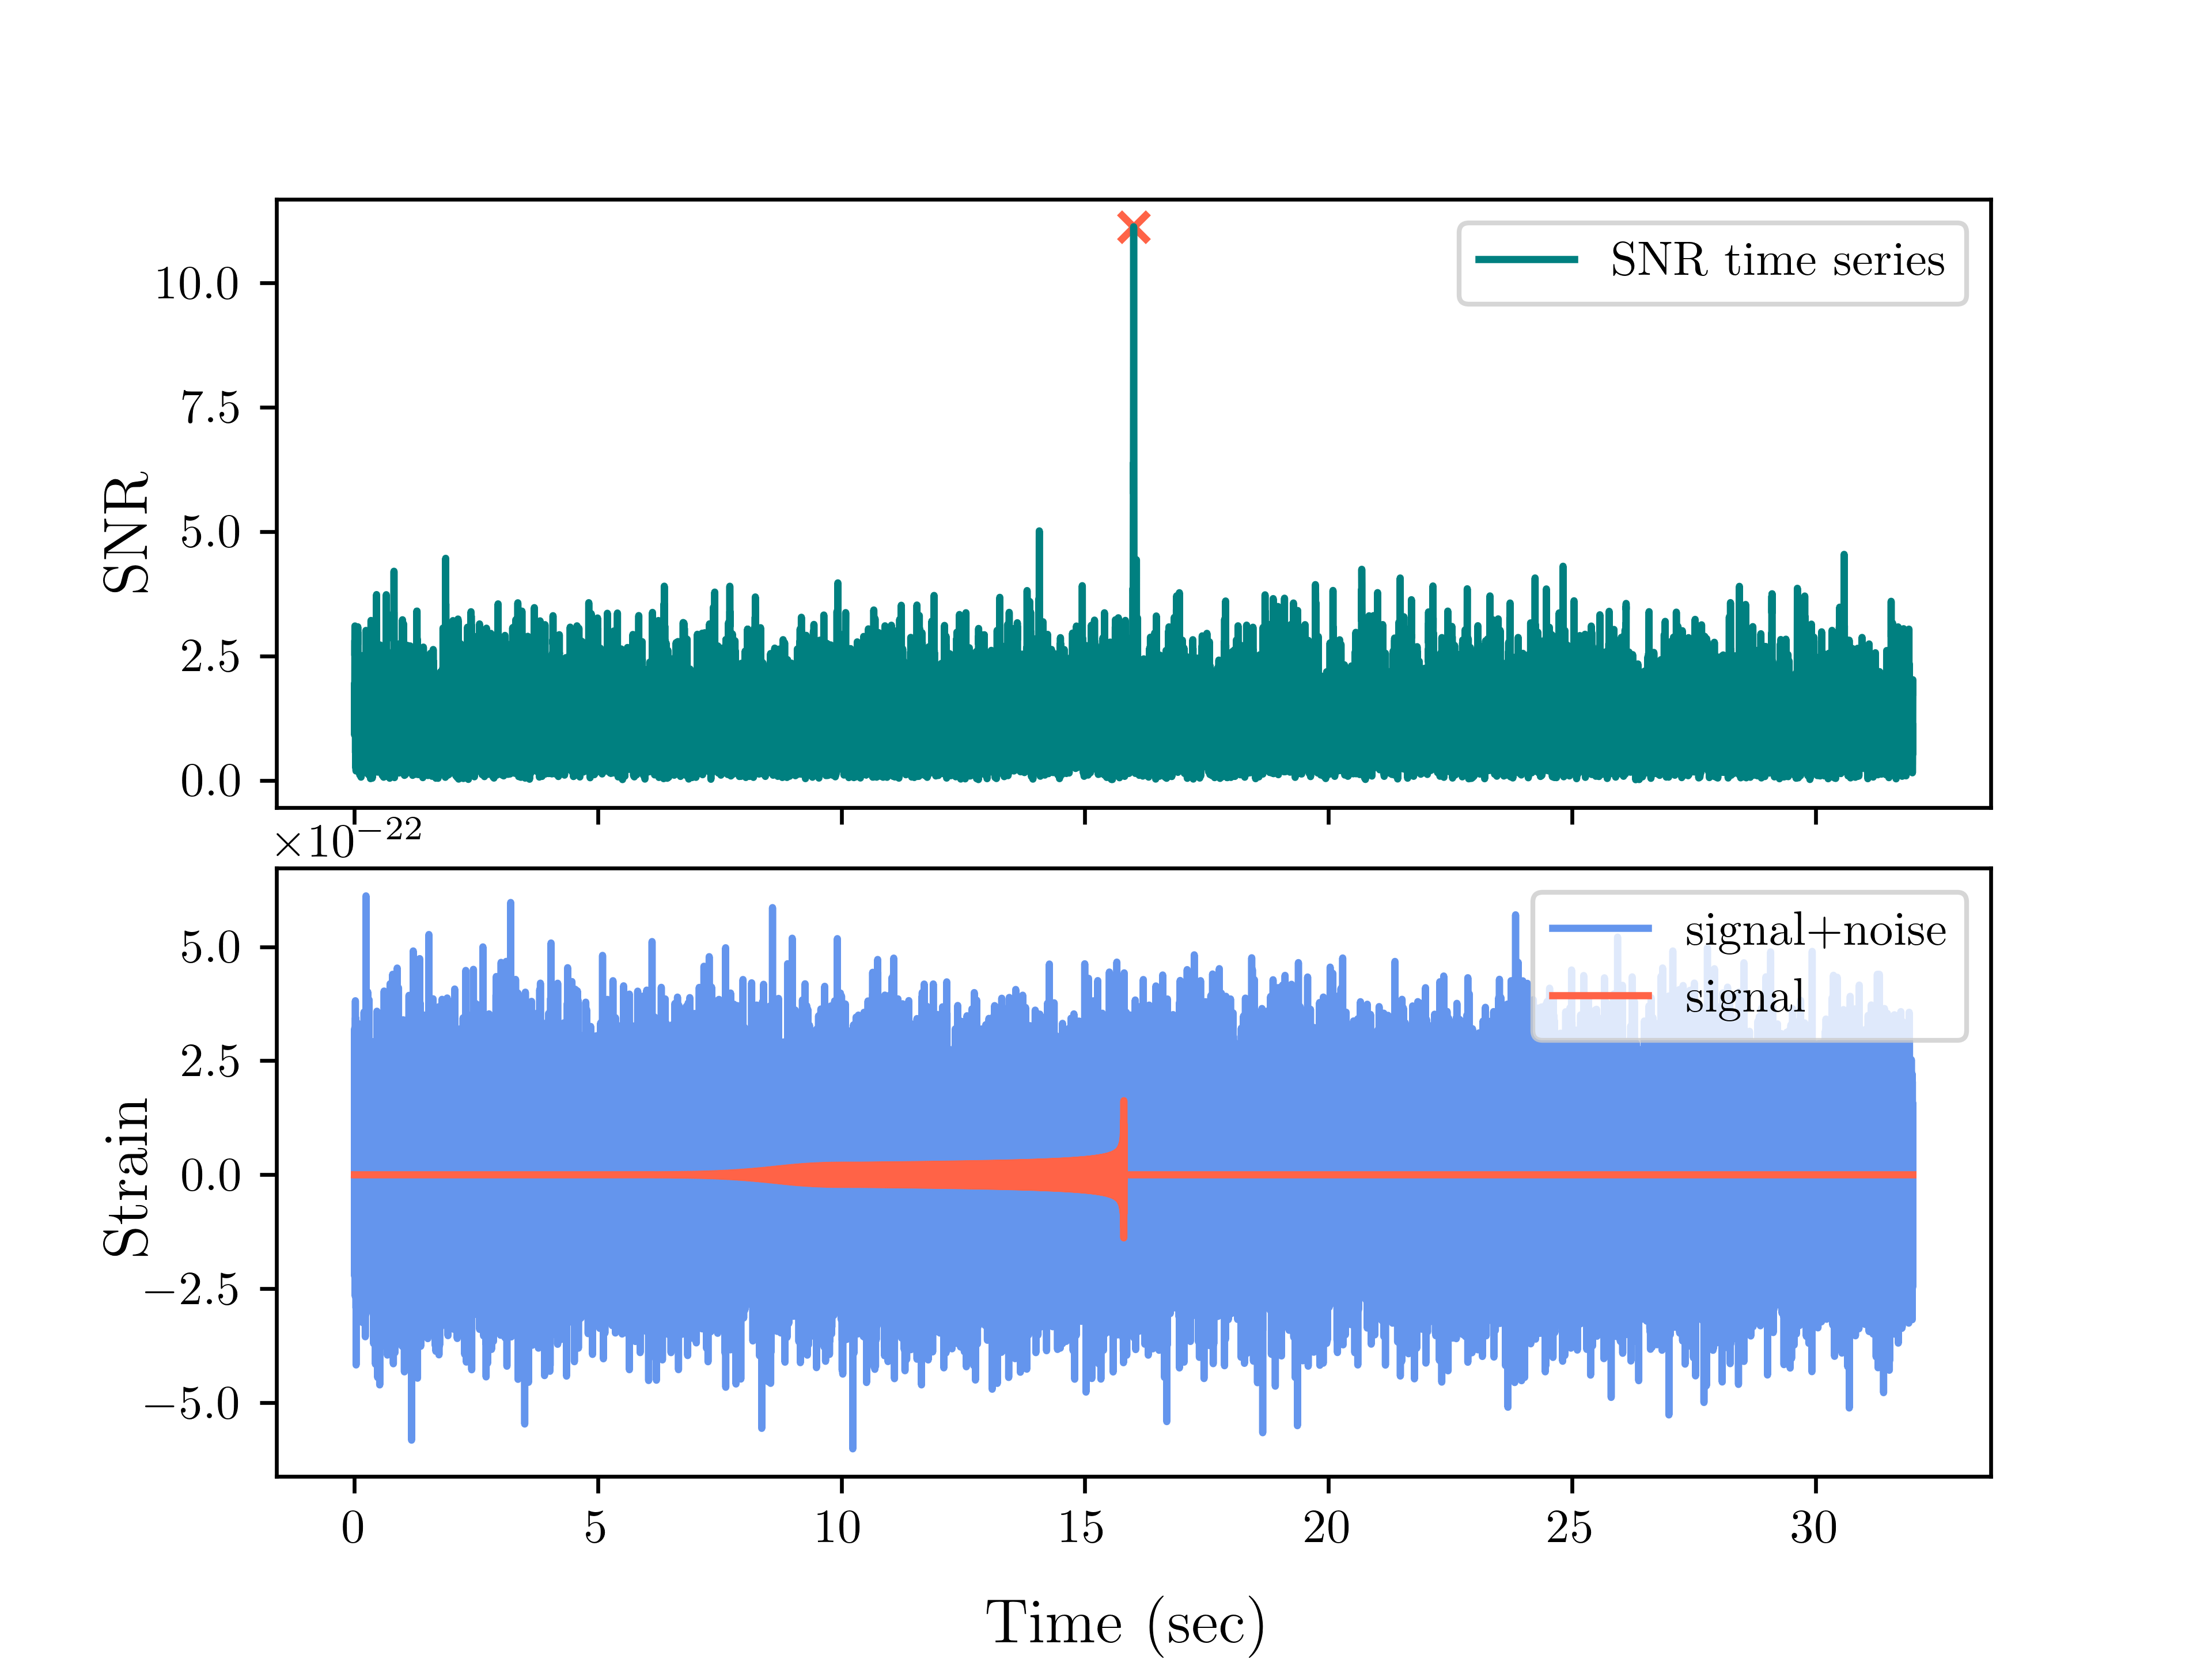
\includegraphics[width=\textwidth]{figures/basic_data_analysis/Matched_filter.png}
    \caption{Matched-filter in action: Bottom panel shows a stretch of strain data containing Gaussian noise and an injected signal from 10-10$M_{\odot}$ BBH. After convolving the template (with the exact injection parameters) with the data, taking the inverse Fourier transform, and then the absolute value, we obtain the SNR time-series as shown in the upper panel. The SNR is sharply peaked at time of the coalescence of the injected signal.}
    \label{fig:Mf-in-action}
\end{figure*}


\section{Detection in non-Gaussian noise}
In scenarios of stationary Gaussian noise, the matched-filter SNR serves as the optimal detection measure. However, when dealing with real detector noise, which often includes transient instrumental artifacts, SNR becomes less effective. Glitches mimic real GW signals by creating high SNR spurious triggers and reduce our confidence in detecting astrophysical signals.

Waveform consistency tests are employed which involve subtracting the GW waveform from the data to get residuals $d-h$ \cite{Allen:2004gu,Joshi:2022ocr}. If these residuals match Gaussian noise, it validates the signal hypothesis. By re-filtering these residuals over different time or frequency spans, any persistent non-noise elements suggest a poor fit of the model waveform $h$ to the data's non-Gaussian feature, resulting in a lowered SNR of a trigger. 

One way to perform this test involves constructing \textit{chi-squared} test statistic to compare the measured and expected power in different frequency bands \cite{Allen:2004gu}. This is done by dividing the matched-filter into $p$ non-overlapping frequency sub-bands such that the expected matched-filter output is equal in each band as shown in Fig. (\ref{fig:chisq_bins})
\begin{align}
    (\hat{h}|\hat{h})_i &= \int_{f_{i-1}}^{f_i} \dfrac{\hat{h}(f)\hat{h}^*(f)}{S_n(f)} df\\
    & = \dfrac{1}{p},
\end{align}
where $i \in [1, p]$ and $f_0 = 0, f_p = \infty$. Then the chi-squared statistic is the squared sum of the residuals of expected and measured matched-filter in each bin 
\begin{align}
    \chi^2 = p\sum_{i=1}^{p} \Bigg( (s|\hat{h})_i - (s|\hat{h})/p\Bigg)^2.
\end{align}
It can be shown if the data contains only Gaussian noise, then $\chi^2$ statistic is chi-squared distributed with $p-1$ degrees of freedom and variance $\sqrt{2p-2}$. In case of glitches, we expect $\chi^2 \gg \sqrt{2p-2}$ and thus, use this statistic to down-weight the glitch triggers by re-weighting the SNR using 
\begin{align}
    \hat{\rho} = \left\{
    \begin{aligned}
        &\dfrac{\rho}{[(1+(\chi^2)^3)/2]^{1/6}},  &\text{if}\hspace{0.2em}  \chi^2 > 2p-2, \\
        & \rho, & \text{if} \hspace{0.2em} \chi^2 \leq 2p-2.
    \end{aligned}
    \right.
\end{align}

\begin{figure*}
    \centering
    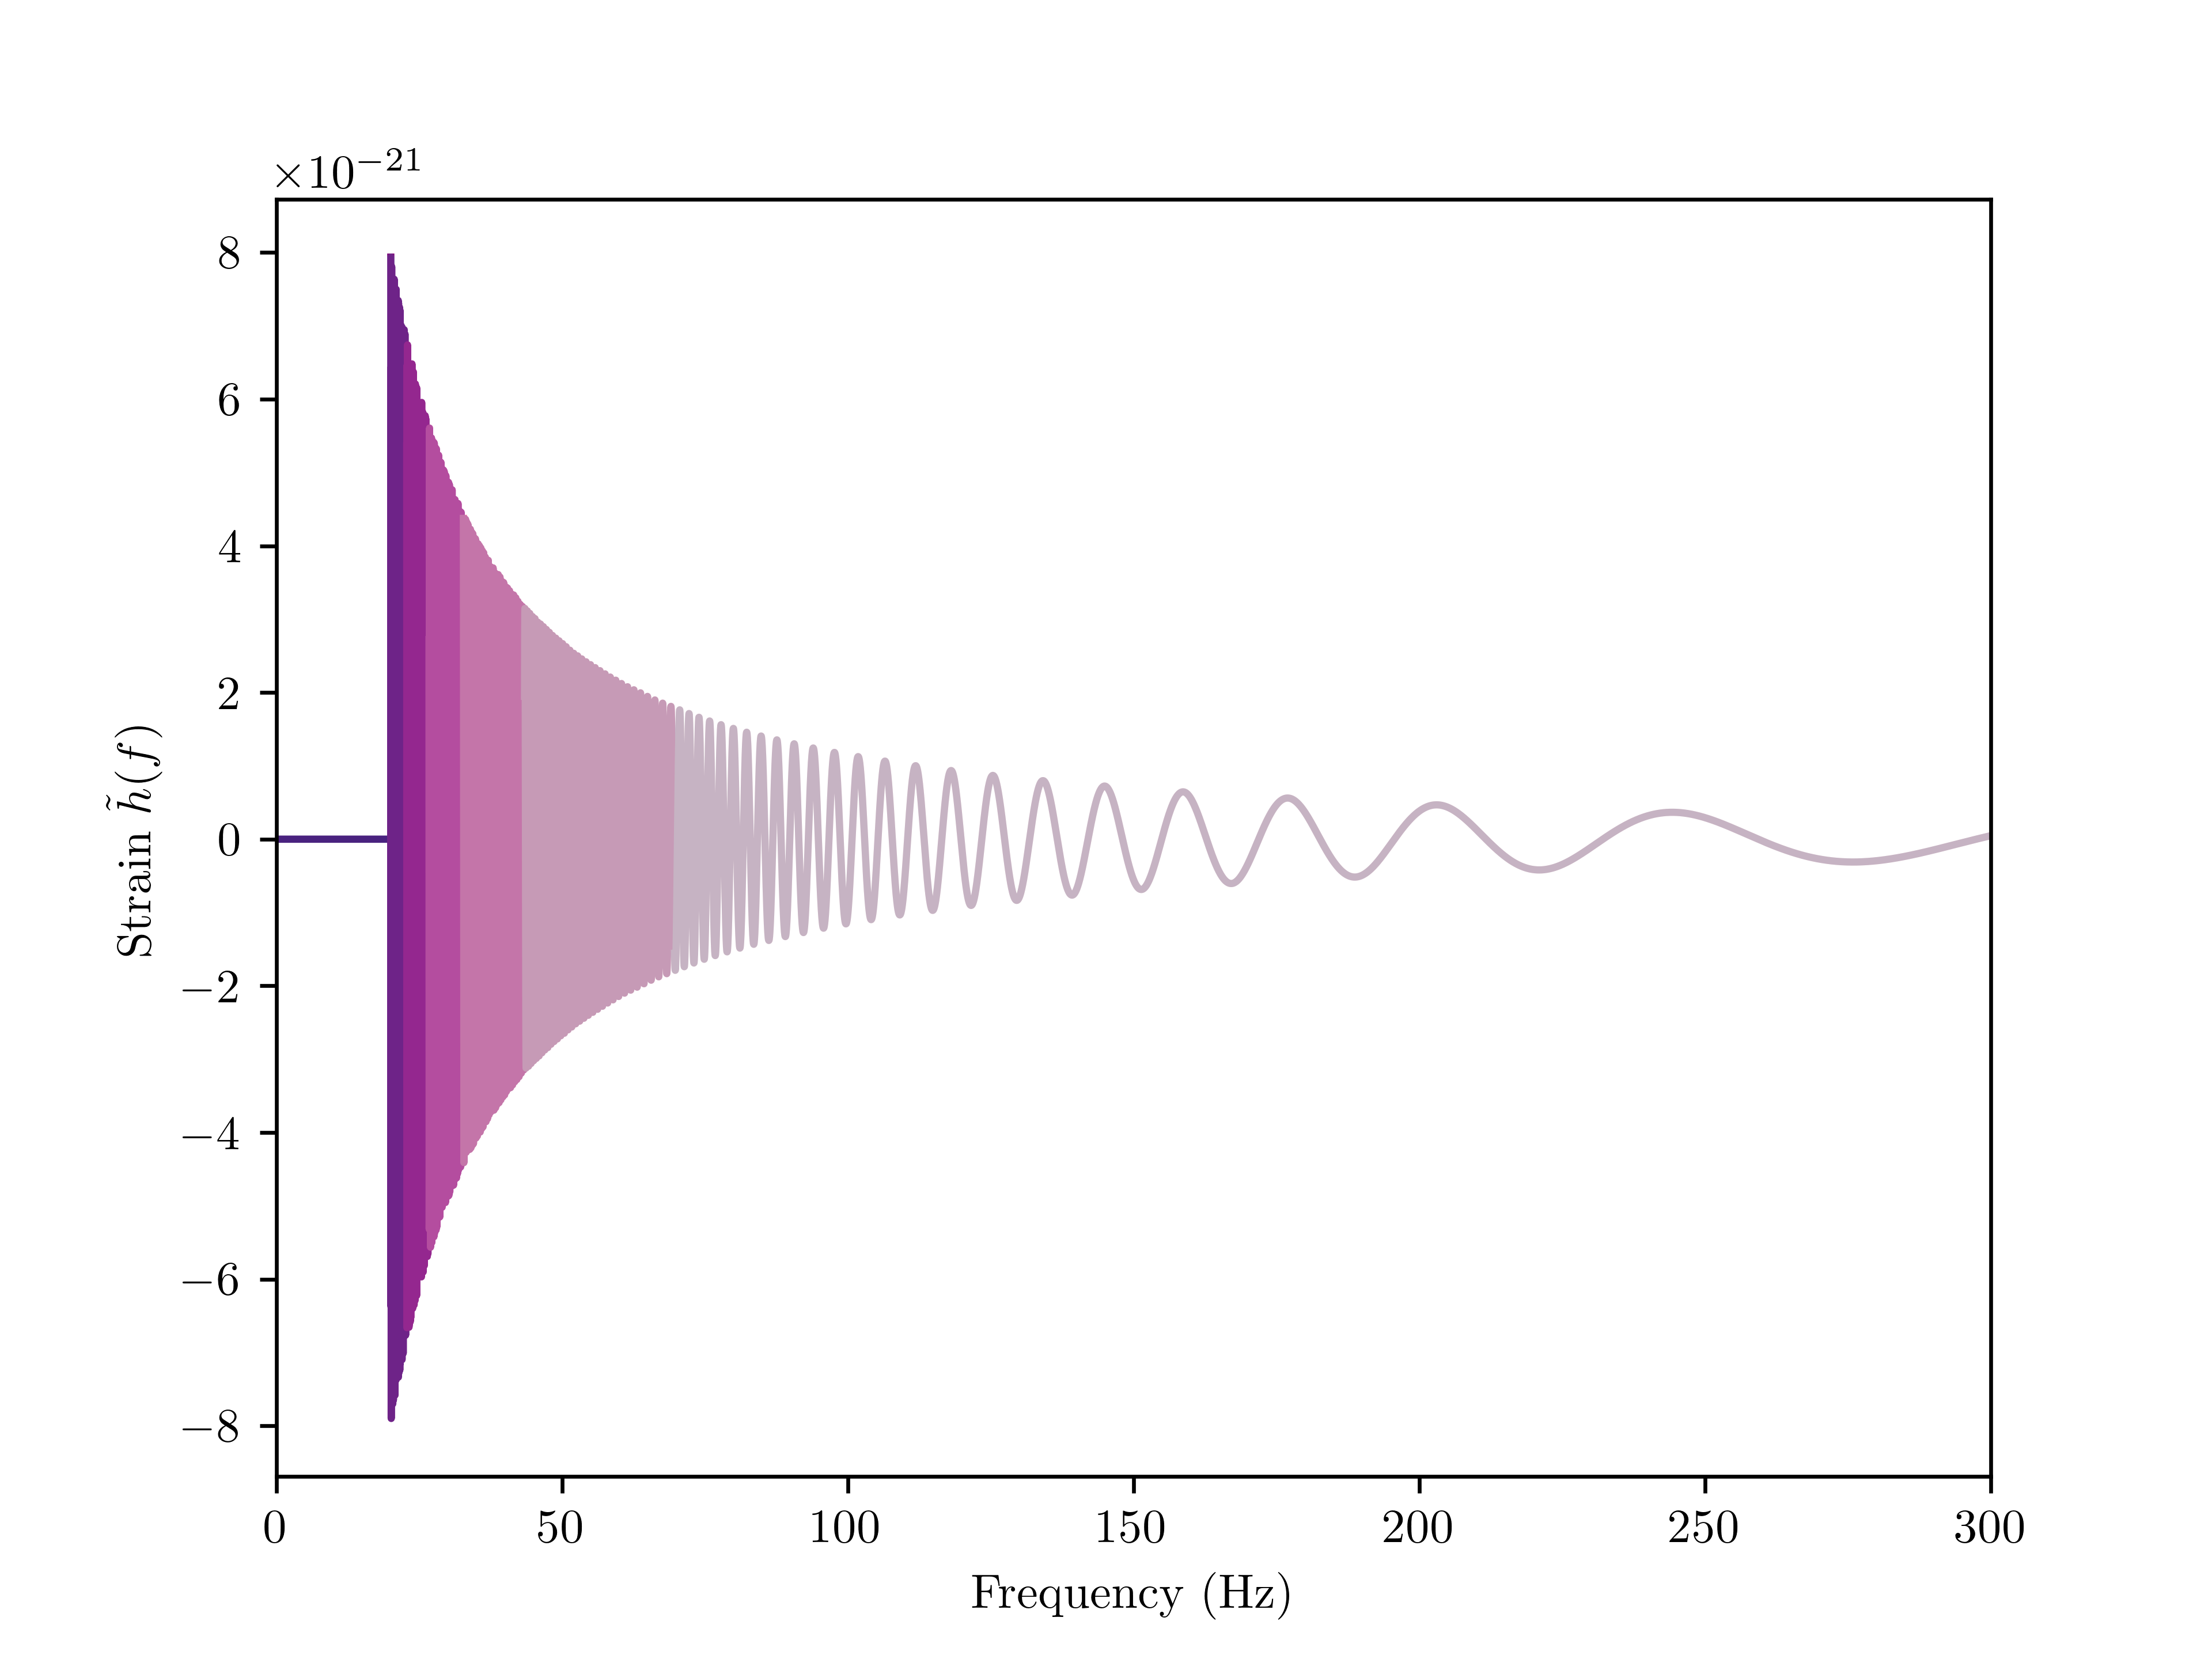
\includegraphics[width=\textwidth]{figures/basic_data_analysis/chissq_bins.png}
    \caption{An example of six frequency bins with equal power used for the $\chi^2$-veto. The signal the amplitude of a Fourier domain signal falls off $\propto f^{-7/6}$, and to maintain the same power in each frequency bin, the frequency bands become wider at higher frequencies, as evident from the plot.}
    \label{fig:chisq_bins}
\end{figure*}

%\subsection{Parameter Estimation}
